\chapter{编写操作系统内核}

从内存管理,输入输出,多进程,分时四个模块丰富操作系统的内容

\section{内存管理}

内存 (RAM) 是计算机中不可缺少的重要硬件,所有程序的运行都是在内存中进行的,
而CPU访问硬盘数据也必须先经过内存交换才得以实现,内存在加速CPU访问硬盘居功至伟。
由内存的重要性可知内存管理在操作系统中也非常重要。	

内存的结构通常用地址和空间表示,在计算机运行过程中,
内存的分配是随机的,导致内存的释放也是相对无序的,这样导致了很多的碎片化问题,
也就是随计算机运行时间变长,内存中到处遍布小块零散空闲空间,虽然零散空间总数很大,
但很难满足新进程序的内存需求,于是内存管理显得十分必要。

内存管理设计的主要目的是快速并且高效的分配内存空间,并在适当的时间释放并回收内存空间。
根据内存管理的设计目的,内存管理的数据结构如下:

\begin{listing}[H]
  \inputminted[tabsize=2, firstline=137, lastline=143,
  linenos=true]{c}{../ZOS/src/kernel/bootpack.h}
\end{listing}

\begin{description}
\item[frees:]空闲空间数量
\item[maxfrees:]用于观察可用状况:frees的最大值
\item[lostsize:]释放失败的内存的大小总和
\item[losts:]释放失败次数
\end{description}

经过内存初始化和释放所有内存空间后,内存管理正常运行。

% memory
\subsection{内存分配}

内存的分配方式与之后的内存释放息息相关,好的分配方式会使得效率大大提高。
根据内存的大小来划分内存如何使用,预计使用32KB用于内存分配的管理空间,
则共有4000组左右的内存用于分配给各个程序使用。

每一组内存经过初始化都拥有自己的数据结构,
即每一组空闲内存的地址和大小都被记录到空闲内存表free。

\begin{table}[!ht]
  \centering
  \begin{tabular}{|c{4cm}|c{8cm}|}
    \hline 
    组号 & 地址 \\
    \hline 
    1 & 0x00003000 \\ 
    \hline 
    2 & 0x00004000 \\
    \hline 
    3 & 0x00005000 \\
    \hline
  \end{tabular}
  \caption{表格示例}
  \label{tab:hello}
\end{table}

一旦系统接收到程序申请内存的请求(需求的内存大小),
就开始在内存中寻找足够大的内存完成这次申请,并返回可供使用的空闲内存的地址。
完成申请后系统需要重新整理空闲内存表free,将最大可用内存组数减一,
将返回给程序空闲空间大小根据程序需求进行调整,并对剩余的可用内存表进行整理。

\begin{listing}[H]
  \inputminted[tabsize=2, firstline=68, lastline=78,
  linenos=true]{c}{../ZOS/src/kernel/memory.c}
\end{listing}

\newpage
\subsection{内存释放}

为保证磁盘空闲空间尽可能少的碎片化,内存释放首先考虑的是使待释放空间与附近空闲空间进行合并。

具体分为三种情况:

\begin{description}
\item[前端空闲:]释放内存的相连前端是空闲内存或释放内存相连两端都是空闲内存
\item[后端可用:]释放内存的相连后端是空闲空间
\item[前端后端均不可用:]挪动空闲空间以合并
\end{description}

已知:待释放的空间的地址和空间大小

根据空闲内存表free的编号查找地址大于待释放空间的空闲内存,
并根据得到的空闲空间编号及大小区分此时的待释放内存应当采取何种方式释放。
\begin{listing}[H]
  \inputminted[tabsize=2, firstline=91, lastline=95,
  linenos=true]{c}{../ZOS/src/kernel/memory.c}
\end{listing}

\newpage
前端空闲:

当待释放的空间前方有空闲空间时,将free[i-1]的大小加上释放空间的大小

内存释放前后情况如图\ref{fig:mem0}和图\ref{fig:mem1}所示: 

\begin{figure}[h]
  \centering
  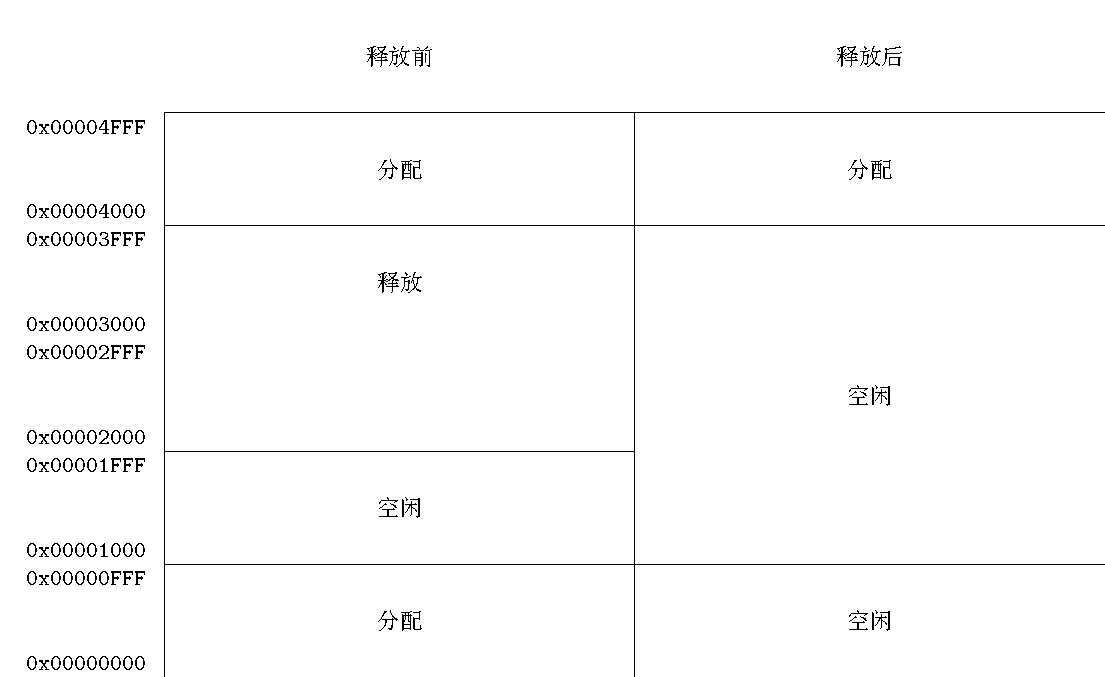
\includegraphics[width=.8\textwidth]{fig/mem0.pdf}
  \caption{前端空闲}
  \label{fig:mem0}
\end{figure}

当待释放的空间后方有空闲空间时,将free[i-1]的大小加上释放空间的大小
\begin{figure}[h]
  \centering
  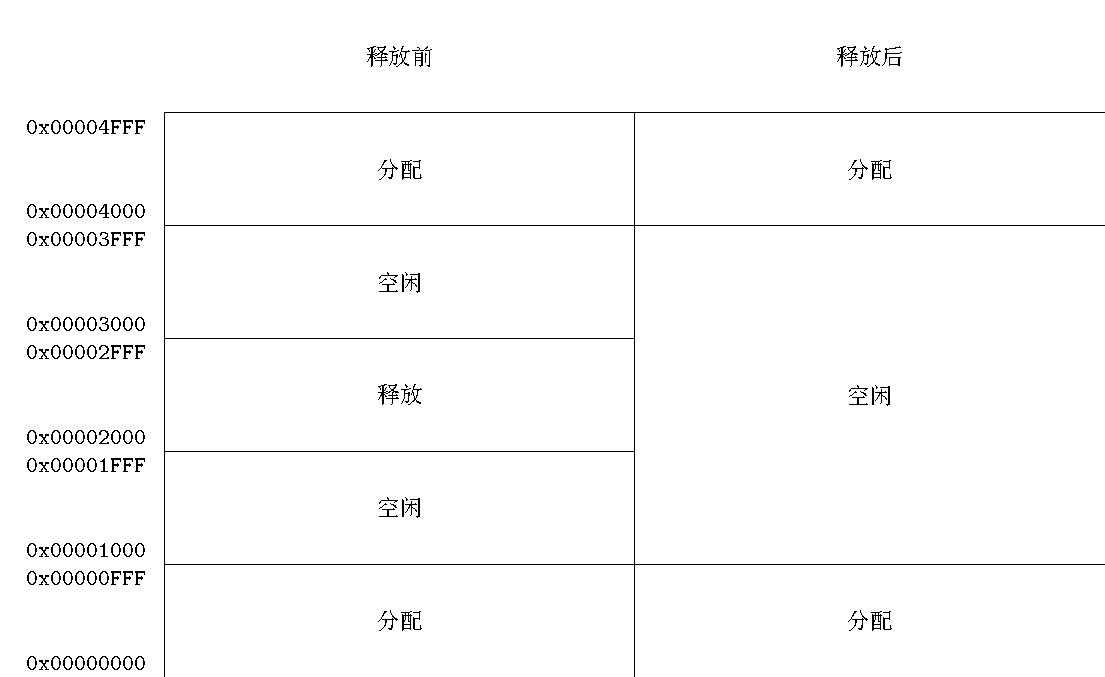
\includegraphics[width=.8\textwidth]{fig/mem1.pdf}
  \caption{前端可用,且后端空闲}
  \label{fig:mem1}
\end{figure}

\newpage
实现如下:

\begin{listing}[H]
  \inputminted[tabsize=2, firstline=98, lastline=116,
  linenos=true]{c}{../ZOS/src/kernel/memory.c}
\end{listing}

\newpage
后端空闲:

内存释放前后情况如图\ref{fig:mem2}所示:

当待释放的空间后方有空闲空间时,将free[i-1]的大小加上释放空间的大小
\begin{figure}[h]
  \centering
  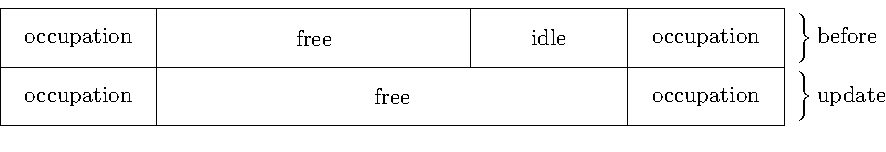
\includegraphics[width=.8\textwidth]{fig/mem2.pdf}
  \caption{后端空闲}
  \label{fig:mem2}
\end{figure}

实现如下:

\begin{listing}[H]
  \inputminted[tabsize=2, firstline=118, lastline=127,
  linenos=true]{c}{../ZOS/src/kernel/memory.c}
\end{listing}

\newpage
前端后端均被占用:

内存释放前后情况如图\ref{fig:mem3}所示:

由于被释放空间周围没有空闲内存,为保证free内各段内存仍然按照内存地址升序排列,
使空闲空间计数最大值加一,free[i]后续空闲内存序号加一,并将释放空间序号定为i。
\begin{figure}[h]
  \centering
  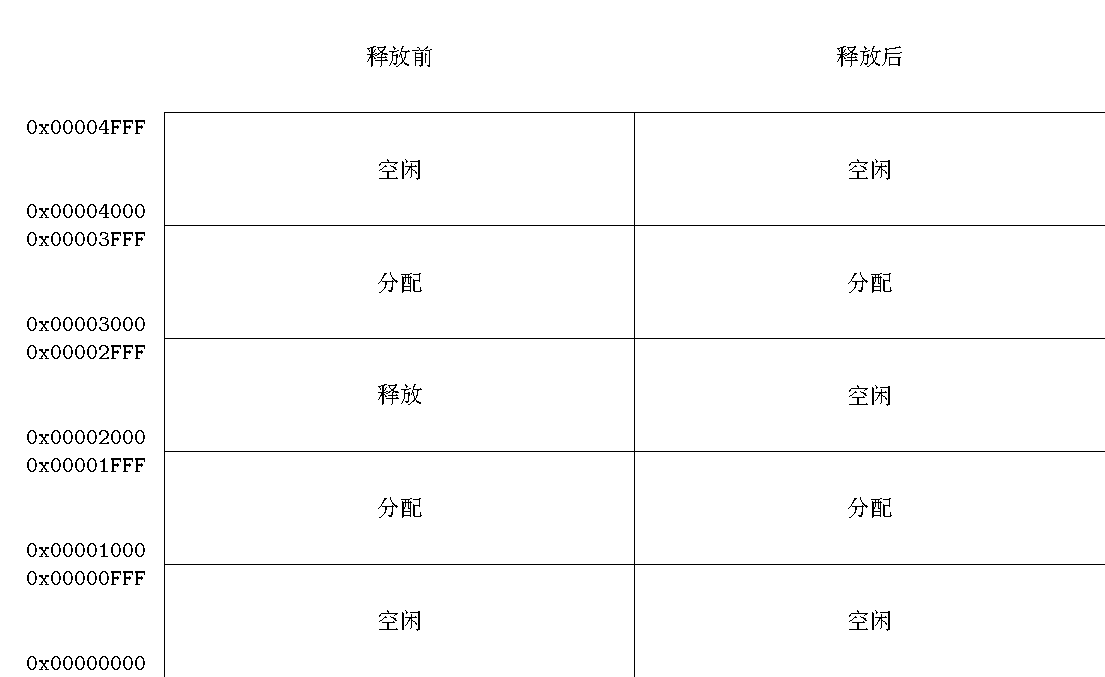
\includegraphics[width=.8\textwidth]{fig/mem3.pdf}
  \caption{前端后端均被占用}
  \label{fig:mem3}
\end{figure}

实现如下:
\begin{listing}[H]
  \inputminted[tabsize=2, firstline=128, lastline=141,
  linenos=true]{c}{../ZOS/src/kernel/memory.c}
\end{listing}

% multi
\documentclass{standalone}
    \usepackage{xeCJK}
    \usepackage{tikz}
    \usetikzlibrary{shapes.geometric, arrows.meta, arrows,positioning}
    
  \begin{document}
  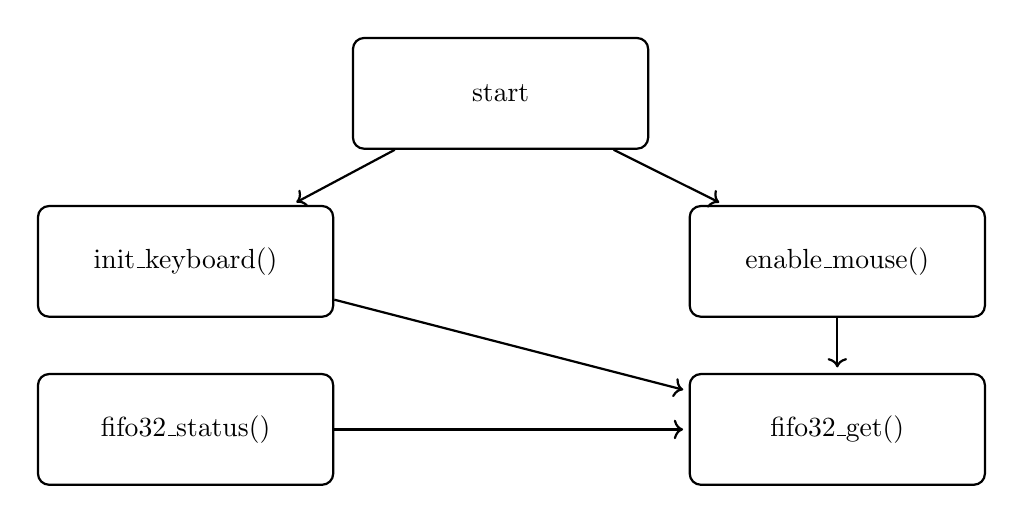
\begin{tikzpicture}
    [auto,
    block/.style={rectangle, draw=black, thick,
    text width=10em,align=center, rounded corners,
    minimum height=4em},
    line/.style={draw, thick, shorten >=2pt, ->}]
  
    \matrix [column sep=5mm,row sep=7mm]
    {
        \node [block] (start) {start}; \\

        \node [block] (init_kbd)[xshift=-4cm]{init\_keyboard()}; & 
        \node [block] (eab_ms)[xshift=1cm]{enable\_mouse()}; \\

        \node [block] (fifo_status) [xshift=-4cm]{fifo32\_status()}; & 
        \node [block] (fifo32_get) [xshift=1cm]{fifo32\_get()}; \\
    };
    \begin{scope}[every path/.style=line]
        \path (start) -- (init_kbd);
        \path (start) -- (eab_ms);
        \path (fifo_status) -- (fifo32_get);
        \path (init_kbd) -- (fifo32_get);
        \path (eab_ms) -- (fifo32_get);
    \end{scope}
    \end{tikzpicture}
\end{document}
  
  %%% Local Variables:
  %%% mode: latex
  %%% TeX-master: t
  %%% End:
  

% multi
\section{多道程序系统}

现代的计算机已经不仅仅作为数字计算的工具,而进入大众生活的计算机被赋予了更多的生活需求,
用户可能在看电影的同时查看电子邮件,也有可能在写论文的时候进入浏览器查询相关资料,
但是更重要的是计算机往往在用户不经意间打开防病毒软件等保证用户计算机的安全\cite{tanenbaum2009modern}。

由此可见多进程的工作方式在计算机工作中不可缺少。

但是在实际的处理过程中,计算机并不能同时处理多个程序,所以必须采用分时的设计,
关于分时操作系统的设计在下一节。
在此有两个概念,同时处理和多个程序,同时处理属于分时,多道程序属于多道程序设计。

首先要处理的问题是如何运行多个程序,早期的多道程序设计的出发点是当时的输入设备是打孔纸带,
CPU速度与输入设备相比差距过大,昂贵的CPU空闲时间就被浪费了,
在A作业等待磁盘或者其他I/O时,CPU暂停为A作业服务,而转向为已I/O操作已完成的B作业服务。

因为A作业和B作业都在计算机中排队,操作员无法区分现在是正在运行的是A作业还是B作业,
但两个作业输出在同一个磁盘,故认为是多道程序在计算机中运行。



% ctss
\section{分时操作系统}

在上一节中说到分时是使得在用户看来计算机的多道程序同时运行,多道程序已经实现了,
分时简单说是使得CPU在用户不能明显感觉到的时间间隔内切换运行多个程序,
在切换后每个程序都能对作业进行一定的处理,在进行多个周期后,各个程序先后完成作业。

不能明显感觉到的时间间隔内切换中有两个概念,时间间隔和切换:

时间间隔太长则用户会有明显的卡顿感,不利于分时概念的实现,
而间隔时间太短则时间不足以让程序响应并完成一定量的工作,同样不利于分时概念的实现。

切换涉及到保存当前程序的运行状态以便于程序获得时间片后可以接续上次的任务继续执行。

